\documentclass{article}
\usepackage{graphicx}
\usepackage{float}

\title{CMSC6950 Project Report: Tidynamics}
\author{Karina Barcelos}
\date{Spring - June 2021}

\setlength{\oddsidemargin}{0.5cm}
\setlength{\textwidth}{15.5cm}
\setlength{\topmargin}{-1.5cm}
\setlength{\textheight}{22cm}

\begin{document}
\maketitle

\section{Introduction}

Tidynamics \cite{Buyl2018} calculates mean-square displacements (MSD) of a trajectory and correlation functions of input data using the Fast Correlation Algorithm. \cite{kneller1995nmoldyn} This package is beneficial for quantitatively evaluating dynamics of stochastic and molecular simulations from numerical trajectories. The autocorrelation function is a correlation of a variable with itself between two successive time intervals (time lags), while mean-square displacement is a deviation of the position of a certain particle regarding a reference position at time intervals. Both funtions are defined by the respective relations below in tidynamics, where the angle brackets denote an average over time. \cite{kneller1995nmoldyn}

The data format input and output of tidynamics \cite{Buyl2018} is array, simply depending only on Python and NumPy. The NumPy arrays where the first index indicates the timestep and the second index, in case of correlation function between two time-series, shows the spatial coordinates of the trajectory. Both ACF and MSD are defined by the respective equations below in tidynamics algorithm \cite{Buyl2018}, where the angle brackets denote an average over time. \cite{kneller1995nmoldyn}

\begin{equation}
C_{AB}(\tau) = \langle A(0) B(\tau) \rangle,
\label{correlation}
\end{equation}
where  $A(0)$ and $B(\tau)$ represent the input data quantity A and the quantity at some later time B, respectively.

\begin{equation}
MSD(\tau) = \langle (x(\tau) - x(0) )^2 \rangle,
\label{msd}
\end{equation}
where $x(\tau)$ and $x(0)$ refer to current and reference positions, respectively.

The aim of this project was to implement two computational tasks of dynamical systems from a chosen open source package such as tidynamics\cite{Buyl2018}. For the first task, the autocorrelation funtion was computed for the bond length of C-H and C=O over 700 ns of a Molecular Dynamics (MD) simulation from a certain Tyrosine amino acid. For the second task,a random walk values and its mean-square displacement were generated. Several modules were utilized during the project, including, numpy, pandas, math, sys, and matplotlib. 

\section{Results}

The results will be reported for use of Autocorrelation funtion and MSD from tidynamics package\cite{Buyl2018}.

\subsection{Task 1: Autocorrelation funtion}

\subsubsection{Example 1: Autocorrelation of C=O and C-H bond length over MD time}

The objective of this task was to analyze the C=O and C-H bond stretching motion using its time autocorrelation function. The input data were obtained from a long MD simulation trajectory with total duration of 1.5 ms of a Tyrosine amino acid of a certain protein. A MD simulation is a computer simulation method that allows to predict and visualize at atomistic level the motion of a system (often a protein) of time evolution. The time evolution herein was in nanosecond (ns) from a period of 800-1500 ns to ensure data analysis in the protein equilibrium. The final input files had the C=O and C-H bond lengths in nanometer (nm) over 700 ns time series and an autocorrelation function calculated from tidynamics \cite{Buyl2018}in a time-series. After load the data, time and length were converted into dataframe. The result after applying the ACF in CH and CO lengths by saving into the same dataframe as well. The resulting txt was a intermediate file for further plotting the Figure \ref{acf_plot}. The ACF showed near zero positive autocorrelation for those non-random length data of those types of bonds, which do not vary drastically over long period of simulation.

\begin{figure}[H]
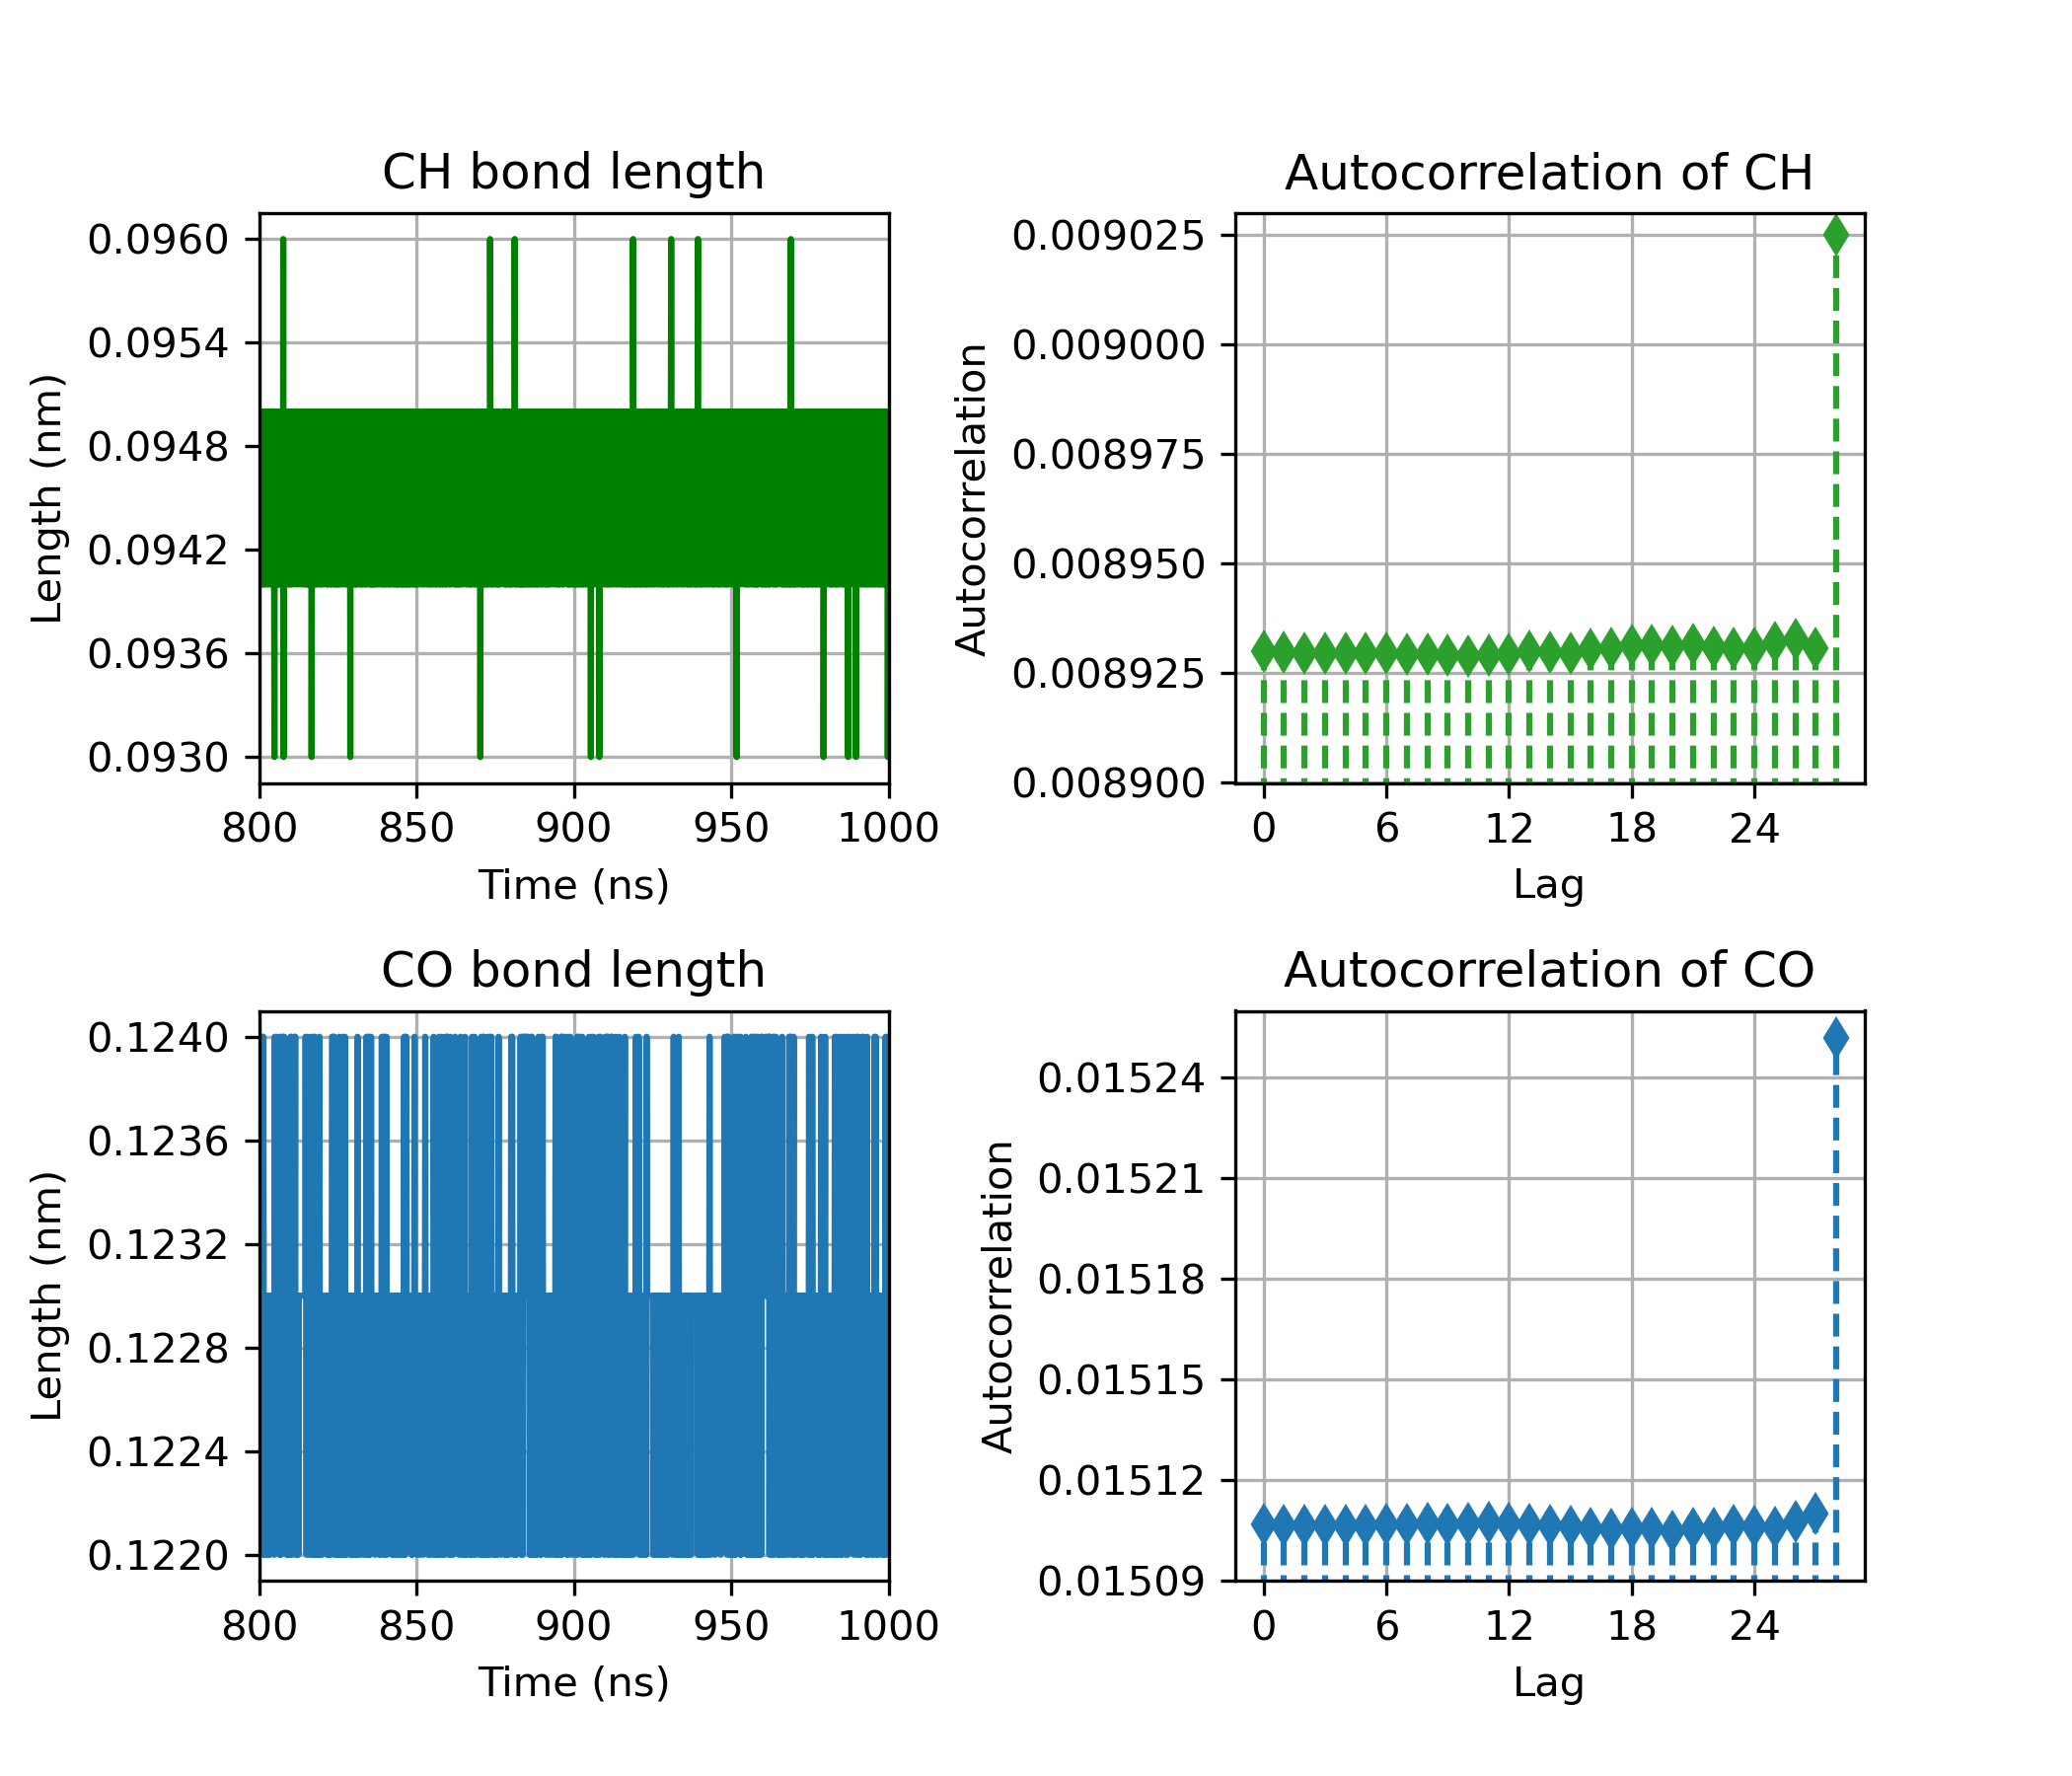
\includegraphics[width=\linewidth]{CO_CH_length_acf_plot.png}
\caption{XXC-H and C=O bond length over Molecular Dynamics time and their autocorrelation function.}
\label{acf_plot}
\end{figure}


\subsection{Task 2: MSD of random walk}

Text

\begin{figure}[H]
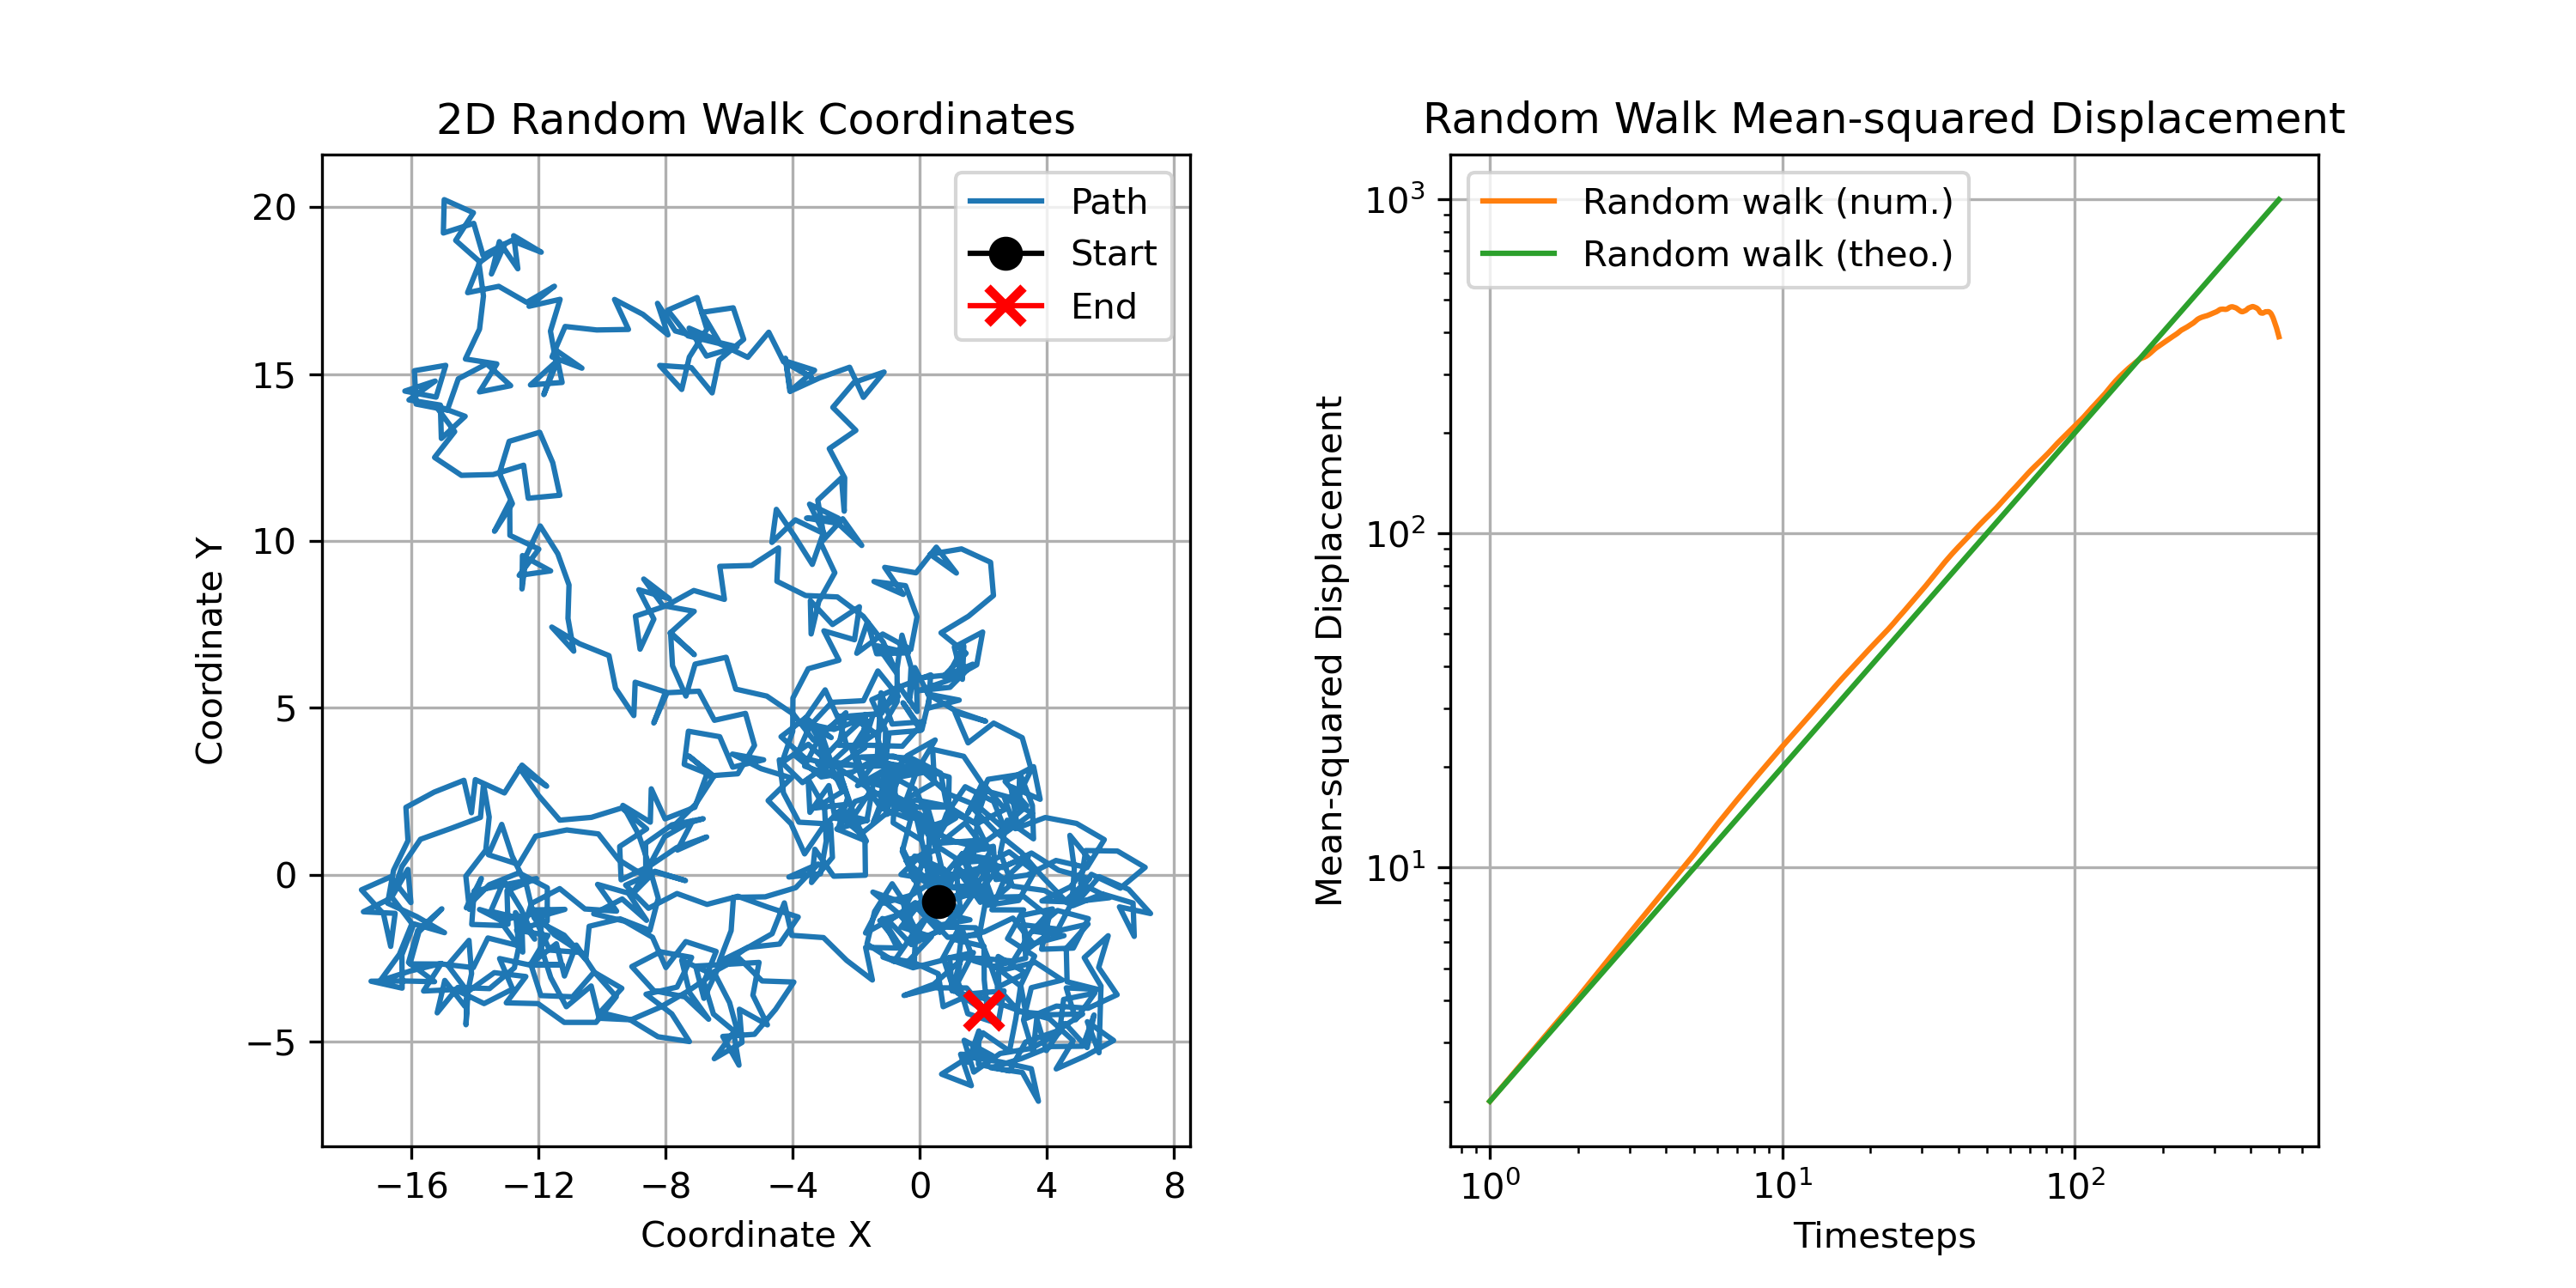
\includegraphics[width=\linewidth]{msd_plot.png}
\caption{2D random walk in a (x,y) coordinates and its mean-squared displacement.}
\label{msd_plot}
\end{figure}



\section{Conclusions}

Therefore, two computational tasks were performed using tidynamics package to calculate a autocorrelation function and MSD and plot their results in different visualizations. The first task provided a visualization from a trajectory of certain protein, wherein the bond length of C-H and C=O over 700 ns a MD dynamics simulation. It required tidynamics, matplotlib, and pandas python libraries. Whereas the second task [continue].

\bibliography{refs}

\end{document}


\bibliographystyle{plain}
\bibliography{references}


\end{document}
